\chapter{Discussion}
Please tell more about conclusion and how to the next work of this study.

\section{Aip Suprapto Munari/1164063}
\subsection{Teori}
\begin{enumerate}
\item Mengapa file suara harus dilakukan MFCC, dilengkapi dengan ilustrasi atau gambar.

Mel Frequency Cepstral Coefficients (MFCC) merupakan koefisien yang merepresentasikan audio. Sehingga diharuskannya melakukan MFCC kepada objek suara atau audio agar suara dapat berubah atau diubah ke dalam bentuk data matrix dimana telah dilakukan ekstraksi oleh MFCC kemudian direalisasikan sebagai data matrix.

\begin{itemize}
\item Ilustrasi Gambar:

\begin{figure}[ht]
\centering
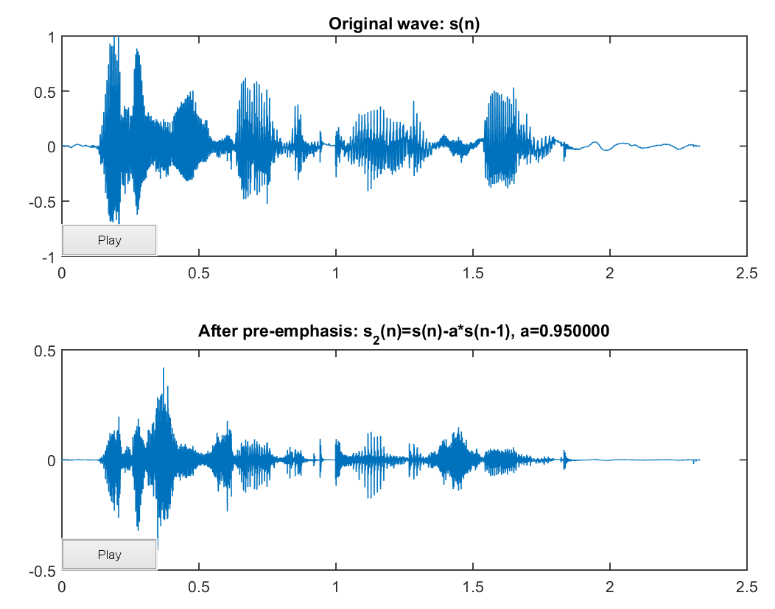
\includegraphics[scale=0.7]{figures/AIP/f1.PNG}
\caption{MFCC - Aip}
\label{MFCC - Aip}
\end{figure}

\end{itemize}

\item Konsep dasar Neural Network, dilengkapi dengan ilustrasi atau gambar.

Neural Network merupakan replika dari sistem syaraf yang terdapat pada sistem otak manusia. Dalam proses kerjanya, otak manusia disusun atas miliaran neuron dimana setiap neuron akan terhubung pada puluhan ribu neuron lain.
\begin{itemize}
\item Ilustrasi Gambar:

\begin{figure}[ht]
\centering
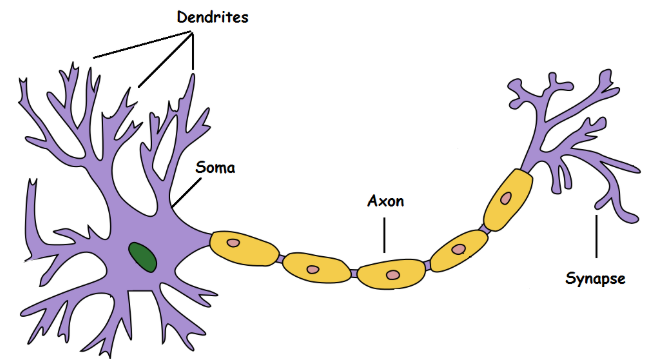
\includegraphics[scale=0.7]{figures/AIP/f2.PNG}
\caption{Konsep Dasar Neural Network - Aip}
\label{Konsep Dasar Neural Network - Aip}
\end{figure}

\end{itemize}

\item Konsep pembobotan Neural Network, dilengkapi dengan ilustrasi atau gambar.

Bobot merupakan suatu nilai yang mendefinisikan tingkat atau kepentingan hubungan antara suatu node dengan node yang lain. Semakin besar bobot suatu hubungan menandakan semakin pentingnya hubungan kedua node tersebut. Bobot merupakan suatu hubungan berupa bilangan real maupun integer, tergantung dari jenis permasalahan dan model yang digunakan. Bobot-bobot tersebut bisa ditentukan untuk berada didalam interval tertentu. selama proses pelatihan, bobot tersebut dapat menyesuaikan dengan pola-pola input.

\begin{itemize}
\item Ilustrasi Gambar :

\begin{figure}[ht]
\centering
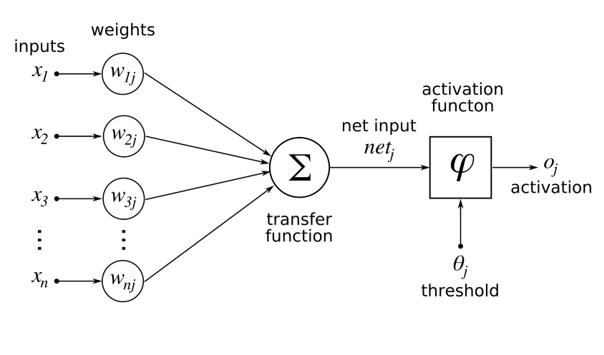
\includegraphics[scale=0.7]{figures/AIP/f3.PNG}
\caption{Konsep Pembobotan Neural Network - Aip}
\label{Konsep Pembobotan Neural Network - Aip}
\end{figure}

\end{itemize}

\item Konsep fungsi aktifasi dalam Neural Network, dilengkapi dengan ilustrasi atau gambar.
Operasi matematik yang dikenakan pada sinyal output y. Sehingga fungsi ini akan digunakan untuk pengaktifan dan juga penonaktifan neuron.
\begin{itemize}
\item Dalam konsep fungsi aktivasi Neuron Network terdapat beberapa jenis:
\begin{itemize}
\item Fungsi Undak Biner Hard Limit ( Menkonversi nilai masukan dari suatu variabel )
\item Fungsi Undak Biner Threshold ( Menggunakan nilai ambang 0 sebagai batas eksekusil )
\item Fungsi Bipolar Symetric Hard Limit ( Mempunyai keluaran bernilai 1 dan 0 )
\item Fungsi Bipolar Threshold ( Mempunyai keluaran bernilai 1, 0 atau -1 )

\item Ilustrasi Gambar:

\begin{figure}[ht]
\centering
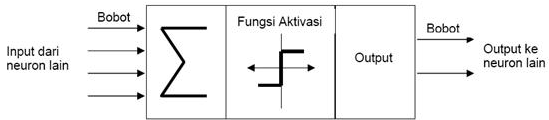
\includegraphics[scale=0.7]{figures/AIP/f4.PNG}
\caption{Konsep Fungsi Aktifasi - Aip}
\label{Konsep Fungsi Aktivasi - Aip}
\end{figure}

\end{itemize}
\end{itemize}

\item Cara membaca hasil plot dari MFCC, dilengkapi dengan ilustrasi atau gambar.

Penjelasan Cara Membaca Hasil Plot Dari MFCC :
\begin{itemize}
\item Ilustrasi Gambar :
\begin{figure}[ht]
\centering
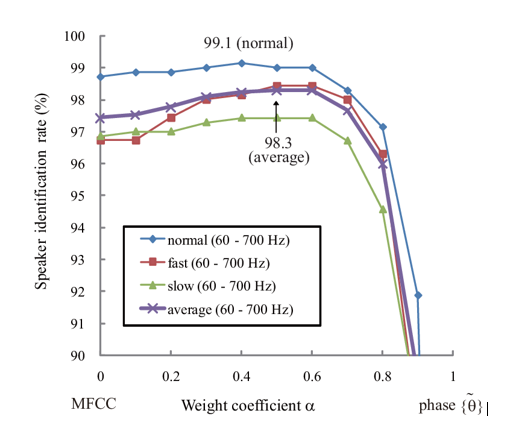
\includegraphics[scale=0.4]{figures/AIP/f5.PNG}
\caption{Plot MFCC - Aip}
\label{Plot MFCC - Aip}
\end{figure}

\end{itemize}

\item Apa itu One-Hot Encoding, dilengkapi dengan ilustrasi atau gambar.


One-Hot Encoding adalah sekelompok bit yang kombinasi hukumnya hanya terdiri dari bit dengan bit tinggi (1) dan bit lainnya rendah (0). Implementasi serupa di mana semua bit '1' kecuali satu '0' kadang-kadang disebut one-cold. Dalam statistik, variabel dummy mewakili teknik serupa untuk mewakili data kategorikal.
\begin{itemize}
\item Ilustrasi Gambar:

\begin{figure}[ht]
\centering
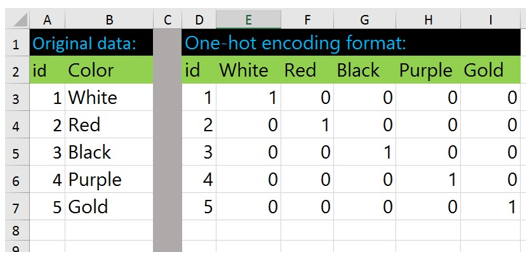
\includegraphics[scale=0.4]{figures/AIP/f6.PNG}
\caption{One-Hot Encoding - Aip}
\label{One-Hot Encoding - Aip}
\end{figure}

\end{itemize}

\item Fungsi dari np.unique dan to.categorical, dilengkapi dengan ilustrasi atau gambar.
\begin{enumerate}
\item np.unique:

Berfungsi untuk menemukan elemen unik array. Ada tiga output opsional selain elemen unik:

\begin{itemize}
\item Indeks array input yang memberikan nilai unik
\item Indeks array unik yang merekonstruksi array input
\item Berapa kali setiap nilai unik muncul dalam array input
\end{itemize}

\item Ilustrasi Gambar :

\begin{figure}[ht]
\centering
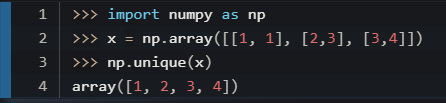
\includegraphics[scale=0.7]{figures/AIP/f7.PNG}
\caption{np.unique - Aip}
\label{np.unique - Aip}
\end{figure}

\item to.categorical:

Berfungsi untuk mengubah vektor kelas yang berupa integer menjadi matriks kelas biner.

\begin{itemize}
\item Ilustrasi Gambar :

\begin{figure}[ht]
\centering
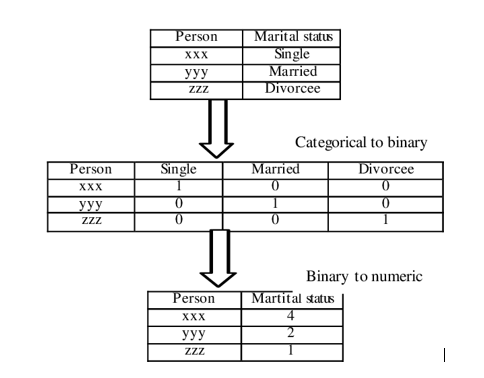
\includegraphics[scale=0.7]{figures/AIP/f7-2.png}
\caption{to.categorical - Aip}
\label{to.categorical - Aip}
\end{figure}

\end{itemize}
\end{enumerate}

\item Fungsi dari Sequential, dilengkapi dengan ilustrasi atau gambar.
Sebuah jenis model yang digunakan dalam perhitungan ataupun code program yang direalisasikan.
\begin{itemize}
\item Ilustrasi Gambar:

\begin{figure}[ht]
\centering
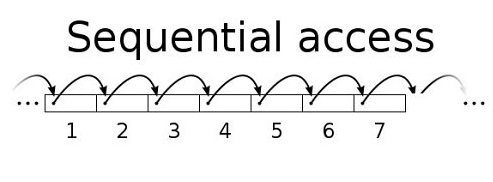
\includegraphics[scale=0.7]{figures/AIP/f8.PNG}
\caption{Sequential - Aip}
\label{Sequential - Aip}
\end{figure}

\end{itemize}
\end{enumerate}
\subsection{Praktek}
\begin{enumerate}
\item Menjelaskan Isi Dari Data GTZAN Genre Colection dan Data Freesound
\begin{itemize}
\par Isi dari data GTZAN adalah data musik berdasarkan genre atau jenis dari lagu.Yang sudah di folderkan berdasarkan jenis lagu nya masing-masing.
\lstinputlisting{src/1164063/1-Aip.py}
\par Hasil \ref{no1Aip} :
\begin{figure}[ht]
\centering
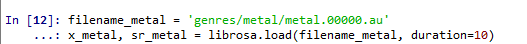
\includegraphics[scale=0.7]{figures/AIP/no1aip.PNG}
\caption{Hasil No 1 Aip}
\label{no1Aip}
\end{figure}
\par Baris 1: filename metal merupakan variabel yang berisikan direktori dari file yang dituju, disini digunakan file audio dari genre metal
\par Baris 2: x metal dan sr metal variabel yang digunakan untuk meload file dari variabel filename metal menggunakan librari Librosa. Yang nantinya akan digunakan pada MFCC
\end{itemize}
\par

\item Menjelaskan Perbaris Kode Fungsi Dari display mfcc()
\begin{itemize}
\item Kode Program
\lstinputlisting{src/1164063/2-Aip.py}
\par Kode Program 2\ref{kodeprogramno2} :
\begin{figure}[ht]
\centering
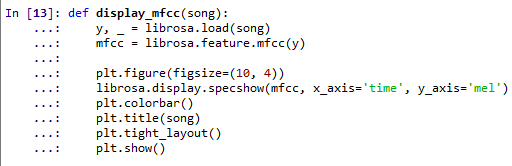
\includegraphics[scale=0.7]{figures/AIP/kd2aip.PNG}
\caption{Kode Program No 2 Aip}
\label{kodeprogramno2}
\end{figure}
\end{itemize}
\begin{itemize}
\item Hasil Plot
\par Apabila Sudah Di Plot \ref{hasil2} :
\begin{figure}[ht]
\centering
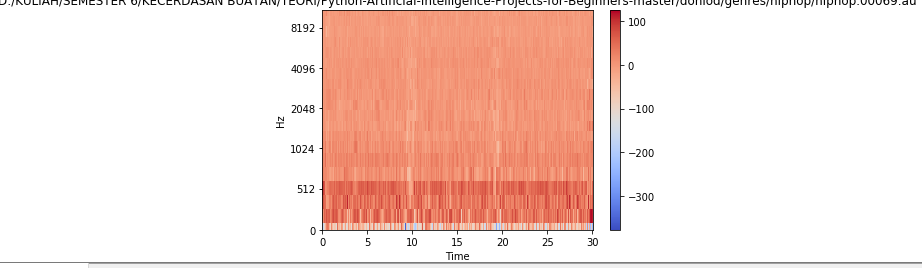
\includegraphics[scale=0.7]{figures/AIP/no2aip.PNG}
\caption{Hasil No 2 Aip}
\label{hasil2}
\end{figure}
\par  Baris 1: Membuat fungsi display mfcc untuk menampilkan vektorisasi sebuah suara
\par  Baris 2: Membuat variabel y untuk membaca variabel song dari perintah library load song
\par  Baris 3: Membuat variabel mfcc untuk variabel y dan mengubah suara menjadi vektor
\par  Baris 4: Memplot gambar dengan ukuran 10X4
\par  Baris 5: Menampilkan spektogram atau chromagram agar hasil dari kodingan ini berwarna atau pada grafiknya
\par  Baris 6: Menambahkan colorbar pada plot
\par  Baris 7: Menetapkan judul suara atau lagu
\par  Baris 8: Memberikan label pada sumbu di grafik
\par  Baris 9: Menampilkan hasil plot
\end{itemize}
\par

\item Menjelaskan Kode Program extract features song() dan Mengapa Yang Diambil 25000 Baris Pertama
\begin{itemize}
\item Penjelasan Kode program
\lstinputlisting{src/1164063/3-Aip.py}
\par Hasil 3\ref{hasil3} :
\begin{figure}[ht]
\centering
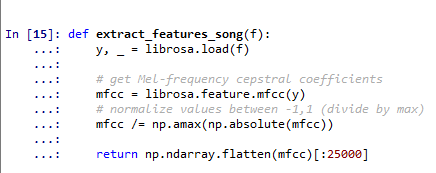
\includegraphics[scale=0.7]{figures/AIP/no3aip.PNG}
\caption{Hasil No 3 Aip}
\label{hasil3}
\end{figure}
\par Baris 1: Membuat fungsi extract features song dengan inputan f
\par Baris 2: Membuat variabel y untuk meload inputan f dari perintah librosa load song
\par Baris 3: Membuat variabel mfcc untuk membuat featuredari variabel y
\par Baris 4: Membuat normalisasi nilai antara -1 sampai 1
\par Baris 5: Mengambil 25000 data pertama berdasarkan durasi suara lalu dikembalikan salinan arraynya  dan dikecilkan menjadi satu.
\item Mengapa Yang Diambil 25000 Baris Pertama
\par Diambil 25000 baris pertama karena agar eksekusi data atau saat running tidak memakan waktu yang cukup lama.
\end{itemize}

\item Menjelaskan Kode Program generate features dan labels 
\begin{itemize}
\item Penjelasan Kode program
\lstinputlisting{src/1164063/4-Aip.py}
\par Hasil 4\ref{hasil4} :
\begin{figure}[ht]
\centering
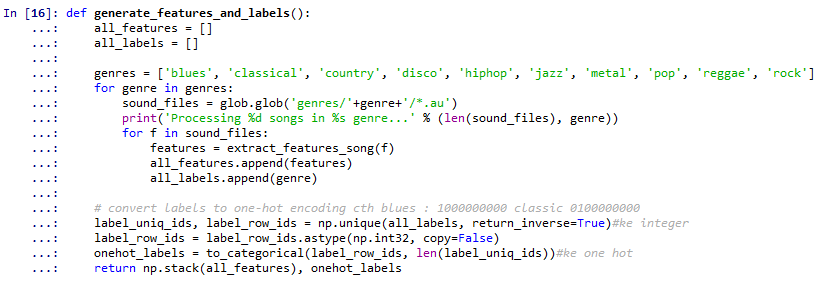
\includegraphics[scale=0.7]{figures/AIP/no4aip.PNG}
\caption{Hasil No 4 Aip}
\label{hasil4}
\end{figure}
\par Baris 1: Pembuatan perintah untuk fungi generate geatures dan labels
\par Baris 2: Membuat variabel all features dengan array / parameter kosong
\par Baris 3: Membuat variabel label dengan array / parameter kosong
\par Baris 4: Mendefinisikan variable genres yang didalamnya berisi nama folder-folder pada variabel genres tersebut
\par Baris 5: Membuat perintah looping ( header )
\par Baris 6: Membuat atribut sound files yang berisi perintah looping perfolder dari folder genres dan mengambil semua file berekstensi au ( semuanya dieksekusi berdasarkan module glob ).
\par Baris 7: Menampilkan jumlah song yang dieksekusi.
\par Baris 8: Membuat perintah fungsi dari sound files
\par Baris 9: Membuat variabel features untuk memanggil fungsi extract features song (f) sebagai inputan. Setiap satu file array sound files dilakukan ekstrak fitur.
\par Baris 10: Memasukkan semua features menggunakan perintah append kedalam all features
\par Baris 11: Memasukkan semua genres menggunakan perintah append ke dalam all labels
\par Baris 12: Mendefinisikan label uniq ids dan label row ids sebagai variabel dimana mengeksekusi perintah np.unique dengan parameter variabelnya all labels dan return inverse=True.
\par Baris 13: Membuat variabel label row ids untuk menentukan type dari variabel tersebut dengan type bit yang sesuai dengan yang digunakan.
\par Baris 14: Membuat variabel onehot labels dimana mengeksekusi to categorical dengan variabel parameter low row ids dan len(label uniq ids)
\par Baris 15: Mengembalikan dan menampilkan hasil eksekusi dari variabel parameter all features dan onehot labels perintah dari np.stack.
\end{itemize}
\par
\par
\item Menjelaskan Mengapa Fungsi generate features and labels sangat lama ketika meload dataset genre
\begin{itemize}
\item Kenapa saat load dataset genre lama? karena ada 1000 data yang di proses.
\lstinputlisting{src/1164063/5-Aip.py}
\par Hasil \ref{no5Aip} :
\begin{figure}[ht]
\centering
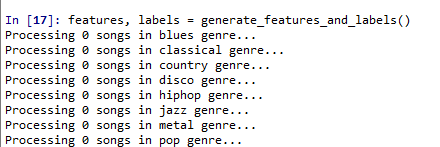
\includegraphics[scale=0.7]{figures/AIP/no5aip.PNG}
\caption{Hasil No 5 Aip}
\label{no5Aip}
\end{figure}
\item Penjelasan Hasil:
\par Baris 1: Variabel features and label akn mengeksekusi isi dari features and label
\par Baris 2: Memproses 100 lagu di genre blues
\par Baris 3: Memproses 100 lagu di  genre classical
\par Baris 4: Memproses 100 lagu di  genre country
\par Baris 5: Memproses 100 lagu di  genre disco
\par Baris 6: Memproses 100 lagu di  genre  hip hop
\par Baris 7: Memproses 100 lagu di  genre jazz
\par Baris 8: Memproses 100 lagu di  genre metal
\par Baris 9: Memproses 100 lagu di genre pop
\par Baris 10: Memproses 100 lagu di genre reggae
\par Baris 11: Memproses 100 lagu di genre rock
\end{itemize}
\par
\par
\item Mengapa Harus Dilakukan Pemisahan Data Training Dan Data Set Sebesar 80\%?
\begin{itemize}
\item Penjelasan :
\par Diperlukan Pemisahan sebesar 80\% data dikarenakan untuk kemudahan dalam melakukan pengacakan yang dimana untuk komposisinya sendiri sebesar 80\% untuk data training dan 20\% untuk data test ( dari dataset ). Data trainingnya memang diharuskan lebih banyak sehingga pada saat pengacakan yang dilakukan datanya akan berada pada urutan yang berbeda.
\item Code Yang Digunakan :
\par 
\par
\lstinputlisting{src/1164063/6-Aip.py}
\par
\par
\item Penjelasan Perbaris ( Tapi dalam soal tidak diperintahkan namun hanya saya jelaskan ) :
\begin{enumerate}
\item Baris Code 1 : Melakukan Proses Training split dimana akan memisahkan training set sebanyak 80\%
\item Baris Code 2 : Melakukan penumpukan features dan labels yang didefinisikan dalam variabel all\_data
\item Baris Code 3 : Melakukan Pengocokan ( shuffle ) untuk variabel all\_data 
\item Baris Code 4 : Membuat variabel splitidx untuk mengkalikan isi dari variabel all\_data dengan training\_split yang ada.
\item Baris Code 5 : Merealisasikan variabel train dan test dengan all\_data yang telah diproses dengan variabel splitidx
\item Baris Code 6 - 7 : Memisahkan mana yang termasuk data train dan mana yang termasuk data test dengan perintah / pada np.shape kemudian di cetak
\item Baris Code 8 - 9 : Menampilkan isi train dari 2 variabel yaitu train\_input dan train\_labels
\item Baris Code 10-11 : Menampilkan isi test dari 2 variabel yaitu test\_input dan test\_labels
\item Baris Code 12-13 : Mencetak / menampilkan data training dimana terdapat 800 baris dan data test sebesar 200 baris dengan jumlah kolom yang sama yaitu 25010
\par
\end{enumerate}
\item  Ilustrasi Gambar : \ref{pemisahan-data-train-set-Aip} dan  \ref{pemisahan-data-train-set-2-Aip}
\begin{itemize}
\item Penjelasan : 
\par Berdasarkan gambar ataupun hasil dari codingan tersebut, memperlihatkan bahwa data dipisah dan dipecah berpatokan dengan ketentuan 80\%. Untuk hasil pertama data trainingnya ada 800 baris dengan 25000 kolom dan data set sebanyak 200 baris dengan 10 kolom, sedangkan untuk hasil kedua yang telah digabungkan dengan one-hot encoding maka data training terdapat 800 baris dan data set dengan 200 baris namun keduanya memiliki jumlah kolom yang sama yaitu 25010.
\par
\par
\begin{figure}[ht]
\centering
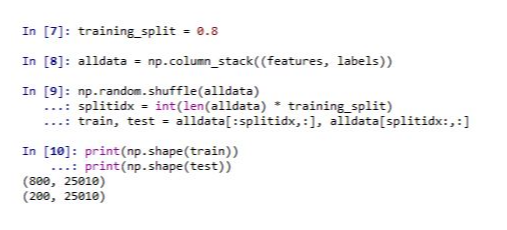
\includegraphics[scale=0.2]{figures/AIP/datatrainset.PNG}
\caption{Pemisahan Data Training Dan Dataset - Aip}
\label{pemisahan-data-train-set-Aip}
\end{figure}
\par
\par
\begin{figure}[ht]
\centering
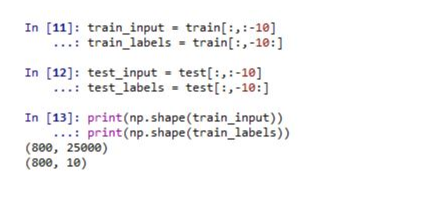
\includegraphics[scale=0.2]{figures/AIP/datatrainset2.PNG}
\caption{Pemisahan Data Training Dan Dataset 2 - Aip}
\label{pemisahan-data-train-set-2-Aip}
\end{figure}
\par
\end{itemize}
\end{itemize}
\par
\par
\item Penjelasan Parameter Dari Fungsi Sequential().
\begin{itemize}
\item Code Yang Digunakan :
\par
\lstinputlisting{src/1164063/7-Aip.py}
\par Penjelasan :
\item Ilustrasi Gambar : \ref{fungsi-sequential-Aip}
\par Pada gambar tersebut dapat dilihat bahwa untuk layer pertama densenya dari 100 neuron kemudian untuk inputan activationnya menggunakan fungsi relu ( nilai maksimum yang akan dipilih ). Dense 10 mengkategorikan 10 neuron untuk jenis genrenya untuk keluarnnya menggunakan aktivasi yaitu fungsi Softmax.
\begin{figure}[ht]
\centering
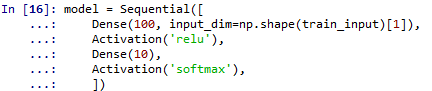
\includegraphics[scale=0.2]{figures/AIP/sequential.PNG}
\caption{Fungsi Sequential - Aip}
\label{fungsi-sequential-Aip}
\end{figure}
\par
\end{itemize}
\par
\par
\item Penjelasan Masing-Masing Parameter Dari Fungsi Compile().
\begin{itemize}
\item Code Yang Digunakan :
\par
\lstinputlisting{src/1164063/8-Aip.py}
\par
\par
\item Ilustrasi Gambar : \ref{fungsi-compile-Aip}
\par
\par Penjelasan :
\par Pada gambar dapat dilihat bahwa untuk model.compilenya dilakukan pemrosesan menggunakan algortima adam sebagai optimizer yang sudah didefinisikan.Kemudian adam tersebut merupakan algoritme pengoptimalan dan untuk memperbarui bobot jaringan yang berulang berdasarkan data training sebelumnya. Untuk loss sendiri menggunakan categorical\_crossentropy yang difungsikan sebagai optimasi skor / accuracy. Dan model tersebut digabungkan serta disimpulkan kemudian dicetak.
\par
\begin{figure}[ht]
\centering
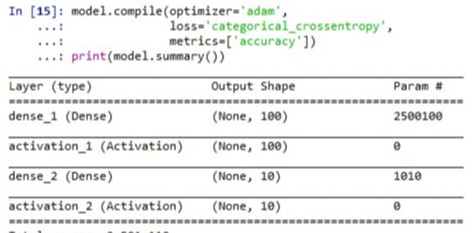
\includegraphics[scale=0.2]{figures/AIP/compile.PNG}
\caption{Fungsi Compile - Aip}
\label{fungsi-compile-Aip}
\end{figure}
\par
\end{itemize}
\par
\par
\item Penjelasan Masing-Masing Parameter Dari Fungsi Fit().
\begin{itemize}
\item Code Yang Digunakan :
\par
\lstinputlisting{src/1164063/9-Aip.py}
\par
\item Penjelasan :
\par Berdasarkan gambar tersebut dapat dilihat bahwa pada model fit dilakukan pelatihan dengan epoch(  iterasi berapa kali nilai digunakan ) dengan rambatan balik sebanyak 10, kemudian dalam sekali epochs dilakukan 32  sampel yang diproses sebelum model diperbarui. Dilakukan validation\_split sebesar 20\% untuk melakukan pengecekan pada cross score validation yang telah dilakukan.
\par
\par
\item Ilustrasi Gambar : \ref{fungsi-fit-Aip}
\par
\begin{figure}[ht]
\centering
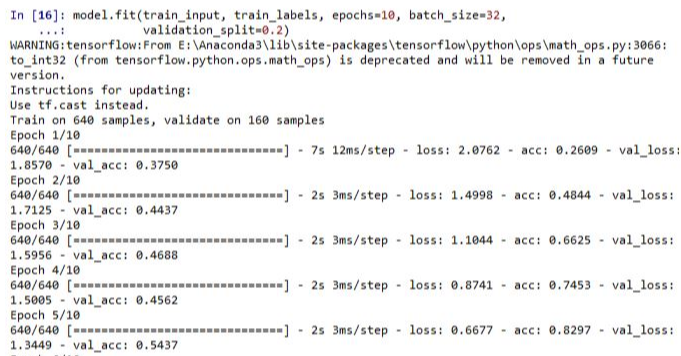
\includegraphics[scale=0.2]{figures/AIP/fit.PNG}
\caption{Fungsi Fit-Aip}
\label{fungsi-fit-Aip}
\end{figure}
\par
\end{itemize}
\par
\par
\item Penjelasan Masing-Masing Parameter Dari Fungsi Evaluate().
\begin{itemize}
\item Code Yang Digunakan :
\par
\lstinputlisting{src/1164063/10-Aip.py}
\par
\item Penjelasan :
\par Berdasarkan code maka dapat dilihat bahwa dengan menggunakan test input dan test label dilakukan evaluasi atau proses menemukan model terbaik yang mewakili data dan seberapa baik model yang dipilih akan dijalankan kedepannya. 
\par Kemudian pada hasilnya sendiri dapat dilihat bahwa Loss merupaka hasil prediksi yang salah sebanyak 1,7985 dan keakurasian prediksinya sebesar 0,4200.
\par
\par
\item Ilustrasi Gambar : \ref{fungsi-evaluate-Aip}
\par
\begin{figure}[ht]
\centering
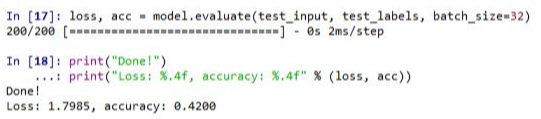
\includegraphics[scale=0.2]{figures/AIP/evaluate.PNG}
\caption{Fungsi Evaluate - Aip}
\label{fungsi-evaluate-Aip}
\end{figure}
\par
\par
\par
\end{itemize}
\item Penjelasan Masing-Masing Parameter Dari Fungsi Predict().
\begin{itemize}
\item Code Yang Digunakan :
\par
\lstinputlisting{src/1164063/11-Aip.py}
\par
\par
\item Ilustrasi Gambar : \ref{fungsi-predict-Aip}
\par Penjelasan :
\par Code tersebut dipergunakan untuk melakukan prediksi diambil dari satu baris berdasarkan test\_input . Nilai yang tertinggi terdapat pada label kedua yang dipilih prediksi yang tepat kemudian akan dikelompokkan.
\par
\par
\begin{figure}[ht]
\centering
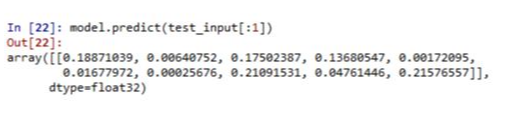
\includegraphics[scale=0.2]{figures/AIP/predict.PNG}
\caption{Fungsi Predict - Aip}
\label{fungsi-predict-Aip}
\end{figure}
\par
\par
\end{itemize}
\end{enumerate}

\subsection{Penanganan Error}
\begin{enumerate}
\lstinputlisting{src/1164063/error-Aip.py}
\item Skrinsut Error
\begin{figure}[ht]
\centering
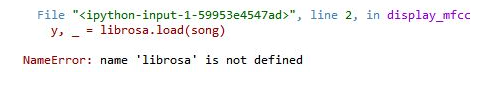
\includegraphics[scale=0.7]{figures/AIP/erroraip.PNG}
\caption{ Error Aip}
\label{6}
\end{figure}
\item Kode Error dan Jenis Errornya
\par Kode Error: "Name Error" name 'librosa' is not defined
\item Penanganan
\par Mendefinisikan library librosa
\end{enumerate}

\section{Andi Muh Aslam}
\subsection{Teori}
\begin{enumerate}
\item Kenapa File Suara Harus Dilakukan MFCC
\begin{itemize}
\item Penjelasan: Agar bisa mengubah suara menjadi vektor. Sehingga data suara bisa diolah menjadi outputan. Jadi semua parameter inputan baik itu suara, dokumen harus dipersiapkan datanya terlebih dahulu, kalau untuk dokumen untuk teks menggunakan word2vec, sedangkan untuk suara menggunakan MFCC (Mel Frequency Cepstral Coeficients) 

\item Ilustrasi Gambar
\begin{figure}[!hbtp]
\centering
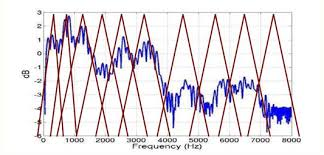
\includegraphics[scale=0.7]{figures/andi/61.jpg}
\caption{MFCC}
\label{Contoh 1}
\end{figure}
\end{itemize}


\item Konsep Dasar Neural Network
\begin{itemize}
\item  Penjelasan:
\par Neural Network merupakan sistem komputasi yang efisien dimana tema utamanya dipinjam dari analogi jaringan saraf biologis. Neural Network biasa disebut dengan jaringan saraf tiruan dimana Neural Network sebenarnya mengadopsi dari kemampuan otak manusia yang mampu memberikan stimulasi/rangsangan, melakukan proses, dan memberikan output.

\item Ilustrasi Gambar
\begin{figure}[!hbtp]
\centering
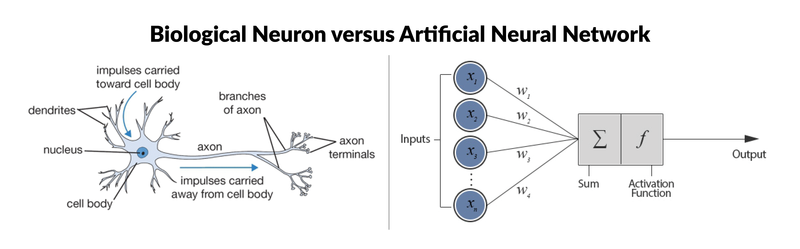
\includegraphics[scale=0.3]{figures/andi/62.png}
\caption{Konsep Dasar Neural Network}
\label{Contoh 2}
\end{figure}

\end{itemize}

\item Konsep Pembobotan Dalam Neural Network
\begin{itemize}
\item Penjelasan:
\par Cara kerja Neural Network dapat dianalogikan sebagaimana halnya manusia belajar dengan mengunakan contoh atau yang disebut sebagai supervised learning. Sebuah Neural Network dikonfigurasi untuk aplikasi tertentu, seperti pengenalan pola atau klasifikasi data, dan kemudian disempurnakan melalui proses pembelajaran. Proses belajar yang terjadi dalam sistem biologis melibatkan penyesuaian koneksi sinaptik yang ada antara neuron, dalam halnya pada Neural Network penyesuaian koneksi sinaptik antar neuron dilakukan dengan menyesuaikan nilai bobot yang ada pada tiap konektivitas baik dari input, neuron maupun output.

\item Ilustrasi Gambar
\begin{figure}[!hbtp]
\centering
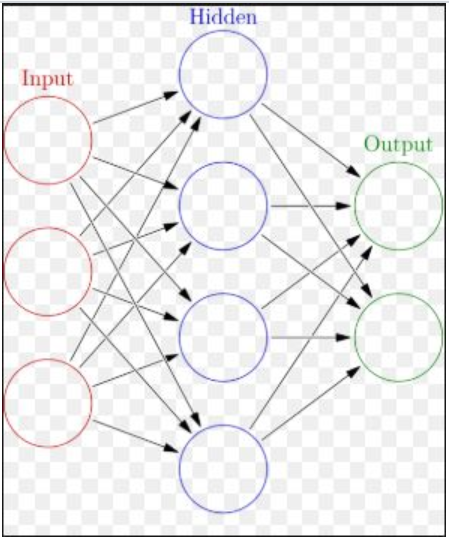
\includegraphics[scale=0.3]{figures/andi/63.PNG}
\caption{Konsep Pembobotan}
\label{Contoh 3}
\end{figure}

\end{itemize}


\item Konsep Fungsi Aktivasi Dalam Neural Network
\begin{itemize}
\item Penjelasan:
\par Setiap neuron mempunyai tingkat aktivasi yang merupakan fungsi dari input yang masuk padanya. Aktivasi yang dikirim suatu neuron ke neuron lain berupa sinyal dan hanya dapat mengirim sekali dalam satu waktu, meskipun sinyal tersebut disebarkan pada beberapa neuron yang lain.

\item Ilustrasi Gambar
\begin{figure}[!hbtp]
\centering
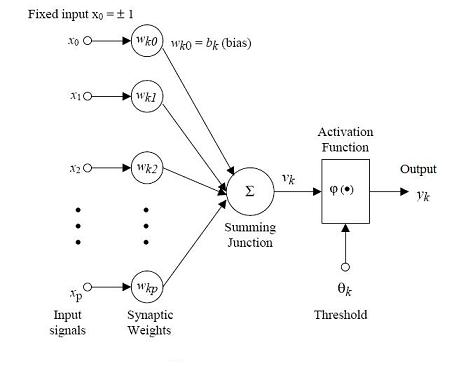
\includegraphics[scale=0.7]{figures/andi/64.jpg}
\caption{Konsep Aktivasi}
\label{Contoh 4}
\end{figure}

\end{itemize}


\item Cara Membaca Hasil Plot Dari MFCC
\begin{itemize}
\item Penjelasan:
\par Cara membaca hasil plot dari MFCC yaitu Nanti akan ada outputan berbentuk grafik setelah melakukan plot dari MFCC. Kemudian terdapat frekuensi/Hz pada suara frekuensi biasanya vertikal atau biasa disimbolkan dengan sumbu y, Lalu terdapat waktu yang mana waktu diartikan dalam simbol sumbu x. Sedangkan pada bagian dalam atau bisa disimbolkan dengan sumbu z merupakan power atau kekuatan dari lagu atau suara atau desibel yang dihasilkan. Untuk warna biru itu merupakan suara rendah, yang merah merupakan tinggi apabila daya frekuensi nya misalkan suara siul berarti dominan warna merah karena siul biasanya pada nada yang tinggi sedangkan jika bass dominan biru karena bass merupakan nada rendah. 

\item Ilustrasi Gambar
\begin{figure}[!hbtp]
\centering
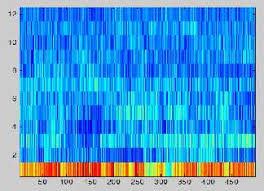
\includegraphics[scale=0.5]{figures/andi/65.jpg}
\caption{Cara Membaca Hasil Plot MLCC}
\label{Contoh 5}
\end{figure}

\end{itemize}




\item Apa Itu One-Hot Encoding?
\begin{itemize}
\item Penjelasan:
\par One-hot encoding adalah representasi dari variabel kategori sebagai vektor biner. Yaitu nilai kategorika harusl dipetakan ke nilai integer. Kemudian, setiap nilai integer direpresentasikan sebagai vektor biner yang semuanya bernilai nol kecuali indeks integer, yang ditandai dengan 1.
\item Ilustrasi Gambar
\begin{figure}[!hbtp]
\centering
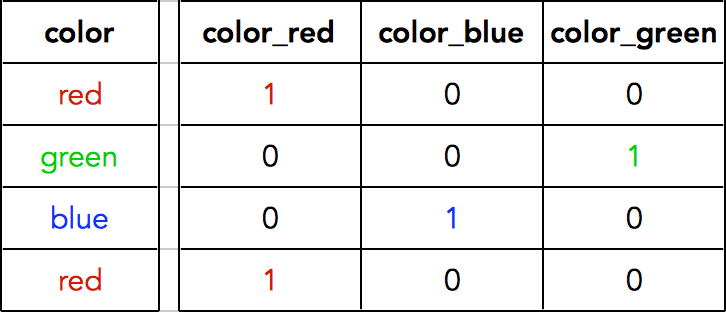
\includegraphics[scale=0.5]{figures/andi/66.png}
\caption{One Hot Encoding}
\label{Contoh 6}
\end{figure}
\end{itemize}


\item Fungsi Dari np unique dan to categorical dalam kode program
\begin{itemize}
\item  Np.unique

\item Penjelasan: np.unique untuk mengekstaksi elemen-elemen unik tertentu dalam array.
\begin{figure}[!hbtp]
\centering
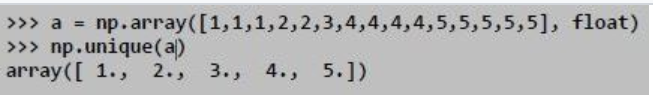
\includegraphics[scale=0.7]{figures/andi/67.png}
\caption{NP Unique}
\label{Contoh 7}
\end{figure}


\end{itemize}
\begin{itemize}
\item  To categorical
\item Penjelasan: Berfungsi untuk mengubah vektor kelas yang berupa integer ( number ) menjadi matriks kelas biner.	
\begin{figure}[!hbtp]
\centering
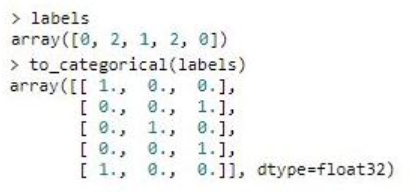
\includegraphics[scale=0.7]{figures/andi/67_1.PNG}
\caption{To Categorical}
\label{Contoh 7_1}
\end{figure}
\end{itemize}


\item Fungsi Dari Sequential Pada Kode Program
\begin{itemize}
\item Penjelasan:
\par Fungsi dari Sequential dalam kode program yaitu meruapakan sebuah jenis model yang digunakan dalam perhitungan ataupun code program yang direalisasikan. Neural Networks Sequential membangun fitur tingkat tinggi melalui lapisan yang berurutan. Sequential juga merupakan proses dimana membandingkan setiap elemen larik satu per satu secara beruntun, mulai dari elemen pertama, sampai dengan elemen terakhir atau elemen yang dicari sudah ditemukan.
\item Ilustrasi Gambar
\begin{figure}[!hbtp]
\centering
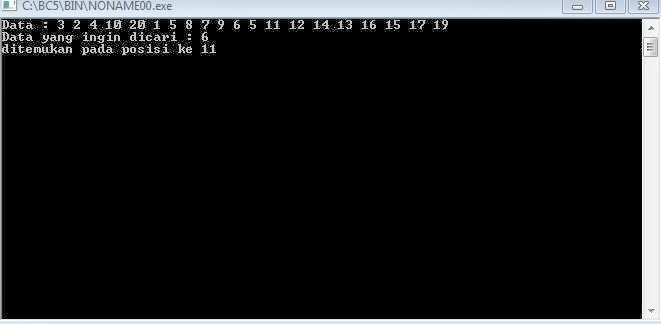
\includegraphics[scale=0.8]{figures/andi/68.jpg}
\caption{Sequential}
\label{Contoh 8}
\end{figure}
\end{itemize}

\end{enumerate}






\subsection{Praktek}
\begin{enumerate}
\item Menjelaskan Isi Dari Data GTZAN Genre Colection dan Data Freesound
\begin{itemize}
\par Dataset GTZAN memiliki 1000 potongan file musik yang berdurasi kurang lebih sekitar 30 detik untuk meload data kita akan menggunakan library python, librosa untuk mengekstrak fitur dari lagu yang terdiri dari 10 kelas genre yaitu blues, classical, country, disco, hip hop, jazz, metal, popular, reggae, dan rock.
\par Hasil :
\begin{figure}[!hbtp]
\centering
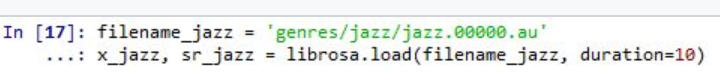
\includegraphics[scale=0.7]{figures/andi/satu.PNG}
\caption{NO 1}
\label{Contoh Gambar 1}
\end{figure}
\par Baris 1: filename jazz merupakan code program untuk memuat inputan data jazz
\par Baris 2: x jazz dan y jazz merupakan variable yang datanya akan di load menggunakan
library librosa, yang nantinya akan di gunakan pada MFCC
\end{itemize}
\par

\item Menjelaskan Perbaris Kode Program Fungsi Dari display mfcc()
\begin{itemize}
\item Kode Program
\par Kode Program 2\ref{dua} :
\begin{figure}[!hbtp]
\centering
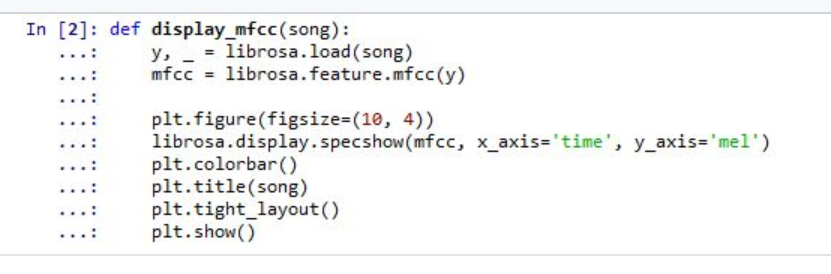
\includegraphics[scale=0.7]{figures/andi/dua.PNG}
\caption{Kode Program No 2}
\label{COntoh Gambar 2}
\end{figure}
\end{itemize}
\begin{itemize}
\item Hasil 
\begin{figure}[!hbtp]
\centering
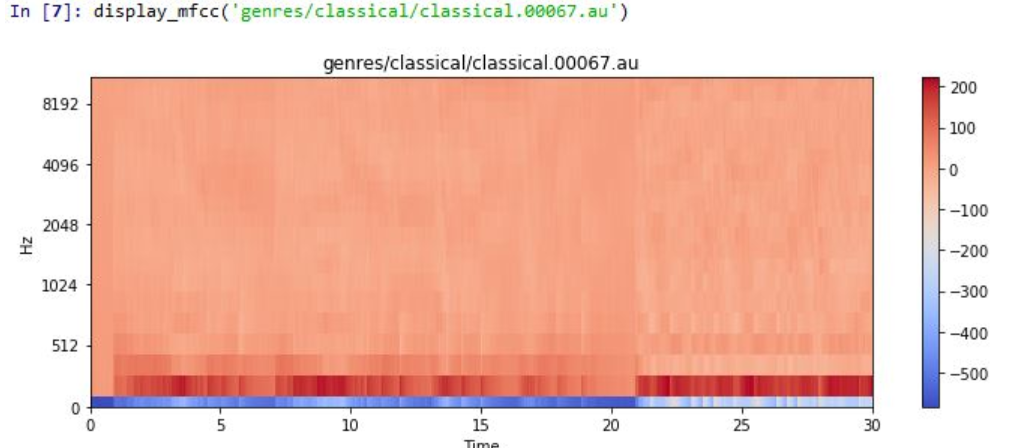
\includegraphics[scale=0.7]{figures/andi/dua2.PNG}
\caption{Hasil No 2}
\label{Contoh gambar 2}
\end{figure}
\par  Baris 1: Untuk menampilkan vektorisasi sebuah suara
\par  Baris 2: membuat variable y agar dapat membaca variable song pada library load song
\par  Baris 3: Untuk mengubah variable y menjadi suara vektor
\par  Baris 4: Mengubah plot gambar dengan ukuran 10x4
\par  Baris 5: Menampilkan Spektogram atau chromagram agar code program dapat berwarna
\par  Baris 6: menambahkan colorbar pada plot
\par  Baris 7: menetapkan judul lagu
\par  Baris 8: memberikan label pada grafik
\par  Baris 9: Menampilkan hasil plot
\end{itemize}
\par

\item Jelaskan Kode Program extract features song(). Mengapa Yang Diambil 25000 Baris Pertama
\begin{itemize}
\item Penjelasan Kode program
\begin{figure}[!hbtp]
\centering
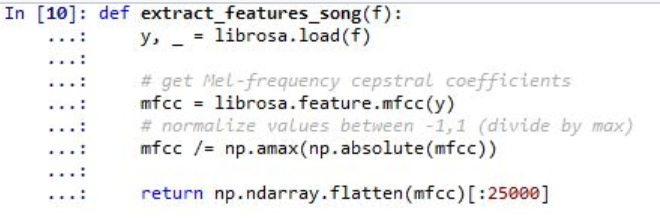
\includegraphics[scale=0.7]{figures/andi/tiga.PNG}
\caption{Hasil No 3}
\label{Contoh Gambar 3}
\end{figure}
\par Baris 1: Membuat fungsi extract features song dengan inputan f 
\par Baris 2: Membuat variabel y untuk meload inputan f dari perintah librosa load song
\par Baris 3: Membuat variabel mfcc untuk membuat feature dari variabel y
\par Baris 4: Membuat normalisasi nilai antara -1 sampai 1
\par Baris 5: Mengambil 25000 data pertama berdasarkan durasi suara lalu dikembalikan salinan arraynya  dan dikecilkan menjadi satu.
\item Mengapa Yang Diambil 25000 Baris Pertama
\par Diambil 25000 baris pertama karena agar eksekusi data atau saat running tidak memakan waktu yang cukup lama.
\end{itemize}
\par

\subsection{Penanganan Eror}
\begin{enumerate}
\item ScreenShoot Error
\item Tuliskan kode eror dan jenis errornya.
\item Solusi pemecahan masalah error tersebut.
\end{enumerate}
\end{enumerate}

